 \section{Конструкторский раздел} \label{desing}

В данном разделе курсовой работы будет рассмотрен процесс проектирования базы данных для разрабатываемого приложения. Будут выделены ключевые этапы проектирования, подробно проанализированы действия в рамках ролевой модели, спроектирован триггер и описаны основные принципы проектирования приложения. Целью данного раздела будет создание базы данных, которая обеспечит стабильную работу приложения и удовлетворит потребности пользователей.


На основе выделенных ранее сущностей спроектированы следующие объекты базы данных.
\begin{enumerate}	
	\item Users --- содержит информацию об участнике и включает следующие поля:
	\begin{itemize}[label=---]
		\item user{\_}id --- уникальный идентификатор пользователя;
		\item token --- авторизационный токен пользователя;
		\item login --- логин пользователя;
		\item name --- имя пользователя;
		\item phone --- телефон пользователя;
		\item rolw --- роль пользователя;
		\item created{\_}at ---  метка времени первой авторизации.
	\end{itemize}
	
	\item Events --- содержит информацию о событиях и включает слудующие поля:
	\begin{itemize}[label=---]
		\item event{\_}id --- уникальный идентификатор события;
		\item name --- название события.
	\end{itemize}
	
	\item Requests --- содержит информацию заявках на участие и включает слудующие поля:
	\begin{itemize}[label=---]
		\item request{\_}id --- уникальный идентификатор заявки;
		\item event{\_}id --- идентификтор конференции, на которую подана заявка;
		\item user{\_}id --- пользователь, подавший заявку;
		\item description --- описание заяки;
		\item status --- статус заявки;
		\item created{\_}at --- метка времени создания заявки;
		\item updated{\_}at --- метка времени обновления заявки.
	\end{itemize}
	
	\item FileMeta --- содержит мета-информация о файлах и включает слудующие поля:
	\begin{itemize}[label=---]
		\item uuid --- уникальный идентификатор файла;
		\item hash --- хеш файла;
		\item created{\_}at -- время загрузки файла.
	\end{itemize}
	
	\item Comment --- содержит информацию о комментариях к заявке
	\begin{itemize}[label=---]
		\item id --- уникальный идентификатор;
		\item request{\_}id --- идентифиматор заявки;
		\item content--- содержимое;
		\item created{\_}at -- время добавления.
	\end{itemize}
	
	\item Aerticle --- содержит информацию о статьях
	\begin{itemize}[label=---]
		\item id --- уникальный идентификатор;
		\item title --- заголовок статьи;
		\item content--- содержимое;
		\item created{\_}at -- время добавления.
	\end{itemize}	
	
	\item File --- содержит информацию об улове участника и включает слудующие поля:
	\begin{itemize}[label=---]
		\item uuid --- уникальный идентификатор файла;
		\item binary{\_}data --- бинарные данные.
	\end{itemize}

\end{enumerate}

Диаграмма проектируемой базы данных представлена на рисунке \ref{fig:er-2}.

\begin{figure}[h!]
	\centering{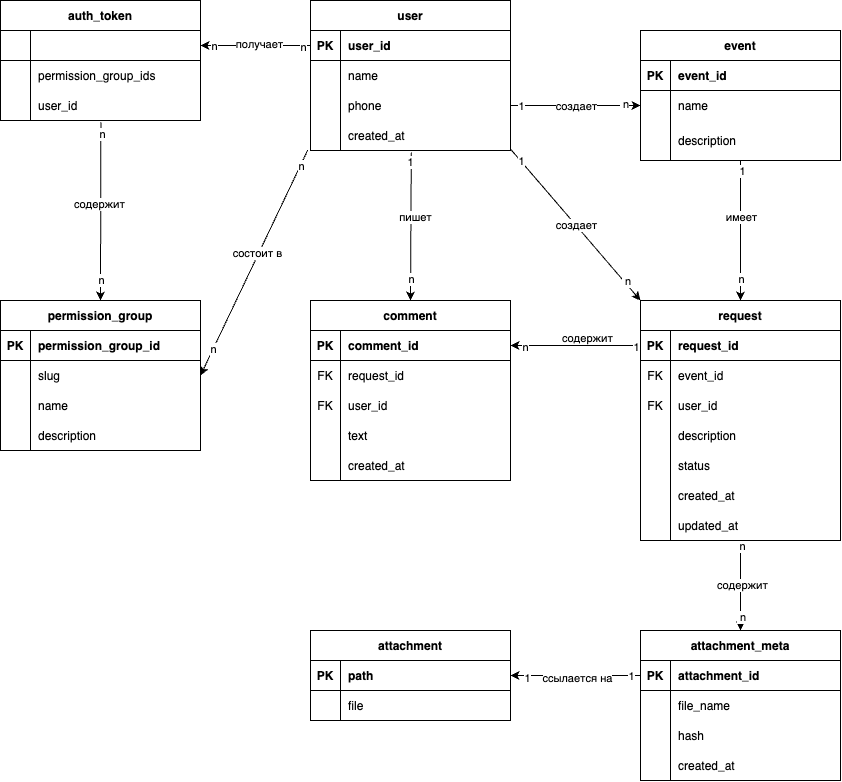
\includegraphics[scale=0.45]{img/er-2.png.png}}
	\caption{Диаграмма проектируемой базы данных}
	\label{fig:er-2}
\end{figure}

\subsection{Ролевая модель}

Ролевая модель предполагает наличие трех ролей: участника, модератора и администратора. Стоит отметить, что модератор обладает всеми правами участника, а администратор --- всеми правами модератора.

Для реализации поставленной выше задачи программа должна предоставлять следующие возможности всем пользователям:
\begin{itemize}[label=---]
	\item авторизация через Yandex OAuth[5];
	\item создание, редактирование заявки на участие;
	\item просмотр списка мероприятий;
	\item добавление приложений к заявке;
	\item просмотр своих заявок;
	\item общение через комментарии к заявке.
\end{itemize}

Модератор также имеет право:
\begin{itemize}[label=---]
	\item просмтаривать все заявки;
	\item создавать, редактировать мероприятия;
	\item изменять статус заявки;
\end{itemize}

Администратор обладаем всеми правами модератора, но кроме того может начначать и удалять модераторов, других администраторов.

\subsection{Триггер}

Триггер — это хранимая процедура особого типа, которую пользователь не вызывает непосредственно, а исполнение которой обусловлено действием по изменению данных: добавлением, модификацией, удалением строки в заданной таблице.

В сущности <<Request>> имеется поле updated{\_}at --- время посоеднего изменения заявки. Также сущность <<заявка>> изменяется при изменении таблицы связи заявки и файла. Для гарантии корректности данного поля и исключения ошибок при update - запросах разумно создать триггер, который будет проставлять данному полю текущее время после совершения операции update над записью, а также после insert, update, delete запсей в таблице связей файла и заявки.

\subsection{Проектиоврание приложения}

При проектиорвании приолжения использован подход <<чистой>>\cite{clean-code} архитектуры, состоящей из следующих слоев:
\begin{enumerate}
	\item слой бизнес логики --- обработка основной логики работы приложения;
	\item слой доступа к данным --- подключение к базе данных, отправка запросов, получение информации из базы данных;
	\item слой программного интерфеса --- обработка запросов от пользователей, делегирование выполнения соответвующим сервисам бизнес-логики.
\end{enumerate}

\subsection{Вывод}

В результате проектирования базы данных для разрабатываемого прило-
жения спроектированы сущности базы данных и их связи, ролевая модель и триггер.

\pagebreak
